\chapter*{Descripciones detalladas de las versiones de poda}
\addcontentsline{toc}{chapter}{Descripciones detalladas de las versiones de poda}

\section*{Poda Alfa-Beta Clásica}
La poda Alfa-Beta clásica es la optimización fundamental del algoritmo Minimax, que utiliza dos cotas, $\alpha$ y $\beta$, para evitar expandir ramas que no pueden alterar la decisión final. $\alpha$ representa la mejor puntuación que puede garantizar el jugador MAX hasta ese momento, mientras que $\beta$ es la mejor puntuación que MIN puede asegurar. Si en algún punto $\alpha \geq \beta$, la rama puede ser descartada de forma segura, ya que no aportará ninguna mejora al resultado global. Esta técnica reduce drásticamente el número de nodos explorados en comparación con el Minimax puro. En este contexto se debe tener en cuenta de no sobrepasar el límite de nodos generados y evaluados, así como el límite de tiempo por movimiento, para garantizar un rendimiento óptimo del agente.

\section*{Poda Alfa-Beta Ordenada}
En esta variante, se incorpora un paso previo de ordenación de los hijos antes de expandirlos. Concretamente, los nodos hijos se ordenan utilizando la heurística (de forma descendente en MAX y ascendente en MIN). La razón de esta mejora es que, si se examinan primero los movimientos más prometedores, las cotas $\alpha$ y $\beta$ se actualizan antes y permiten podar más ramas en niveles superiores, acelerando significativamente la búsqueda. Para su implementación, se utiliza una función de ordenación que prioriza los nodos con mayor puntuación heurística, lo que mejora la eficiencia del algoritmo al reducir el número de nodos explorados. Al ordenarse en base a la heurística, el orden depende fundamentalmente de la calidad de la heurística utilizada, por ende, si la heurística no es del todo correcta y el algoritmo es perfecto, no se va a obtener el resultado esperado (óptimo).

\section*{Poda Alfa-Beta Probabilística}
Esta versión introduce un parámetro de tolerancia $\epsilon$ que relaja el criterio clásico de poda. En lugar de podar sólo cuando $\alpha \geq \beta$, se permite la poda anticipada si la diferencia $\beta - \alpha$ es menor que $\epsilon$. Con esto se asume que es poco probable que la rama mejore significativamente el resultado, y se corta la exploración para ganar velocidad a cambio de una ligera pérdida potencial de calidad en la jugada elegida. Es una técnica especialmente útil para profundizar más sin comprometer demasiado el rendimiento general. La implementación se ha basado fundamentalmente en lo mencionado, si la rama no es ``bastante prometedora'', se poda. Cabe destacar que he optado por un valor de $\epsilon$ de 0.3, el cual es bastante pequeño, pero es que tras numerosas pruebas era el valor que mejor se ajustaba\footnote{También se realizaron pruebas con 0,5 y 0 para ver si con solo la poda alfa-beta y quietud bastaba, pero los resultados eran bastante peores.}.

\section*{Profundidad Dinámica}
La profundidad dinámica adapta la profundidad máxima de búsqueda en función de la cantidad de hijos generados en un nodo. La idea es que, cuando hay pocas opciones (baja ramificación), se puede profundizar más para explorar jugadas con mayor precisión. Por el contrario, cuando hay muchas opciones (alta ramificación), se limita la profundidad para no sobrepasar el número máximo de nodos. Así, se equilibra la carga de cómputo y se aprovechan mejor los recursos disponibles. En este punto pensé en ampliar la profundidad máxima de búsqueda, pero había casos en los que si podía entrar en esa rama y tardar una infinidad de tiempo.

\section*{Búsqueda de Quietud}
La búsqueda de quietud se utiliza para evitar evaluaciones engañosas en estados de juego inestables. Cuando se alcanza la profundidad máxima y el estado no es "quiescente" (hay capturas o movimientos tácticos relevantes inminentes), se siguen explorando exclusivamente esas jugadas tácticas. Así se obtiene una evaluación más realista del estado final. Esto ayuda a mitigar el efecto de los ``horizontes artificiales'' que pueden inducir decisiones erróneas en situaciones críticas.
La lógica comienza evaluando el estado actual como \texttt{stand\_pat\_score}. Si no hay movimientos tácticos, devuelve ese valor directamente. Si los hay, explora recursivamente solo esos hijos tácticos, actualizando los valores \texttt{alpha} o \texttt{beta} y aplicando poda cuando corresponde (\texttt{beta <= alpha}). De esta forma, permite “dejar que se resuelva el caos” antes de tomar decisiones finales, evitando evaluaciones erróneas por cambios bruscos en la posición. Esta búsqueda se detiene cuando se alcanza la profundidad máxima de quietud o se llega a un estado estable.

\section*{Versión Combinada: Poda Alfa-Beta Ordenada, Probabilística y Dinámica}
La versión más avanzada que hemos implementado combina varias de las mejoras anteriores en un único algoritmo. Integra:
\begin{itemize}
    \item La ordenación de los hijos para podar más rápidamente.
    \item La poda probabilística para cortar ramas menos prometedoras de forma anticipada.
    \item El ajuste dinámico de la profundidad según la ramificación del árbol.
    \item Además, utiliza la búsqueda de quietud en los nodos límite para evitar evaluaciones precipitadas.
\end{itemize}
Este enfoque integral permite un equilibrio óptimo entre la calidad de las decisiones y el tiempo de respuesta, maximizando la competitividad del agente frente a adversarios exigentes.
Aunque desde el punto de vista teórico, se ve que funciona correctamente, tras numerosas pruebas, nuestra heurística funcionaba de mejor manera en la implementación del algoritmo de poda alfa-beta probabilística y quietud con un valor de $\epsilon$ de 0.3, es decir, casi despreciable, y con ayuda de la búsqueda de quietud. Gracias a esto se ha logrado vencer $4/6$ casos posibles (3 ninjas, teniendo en cuenta los casos en los que puedo empezar yo o el ninja). \textit{Curiosamente se llego a la conclusión de que en mi caso, y repito, tras numerosas pruebas de heurísticas y valores de las mismas, se podía adoptar ``un cambio dinámico de los valores de la heurística'', lo que se traduce en que si empiezo yo (el id es 0) adopto unos valores determinados y si empieza el ninja (el id es 1) adopto otros valores. Pero esto no se ha implementado debido a que no es lo que se pedía en el enunciado.} 



\chapter*{Búsqueda de Quietud: Motivación y Explicación}
\addcontentsline{toc}{chapter}{Búsqueda de Quietud: Motivación y Explicación}

La búsqueda de quietud es una técnica que se añade a los algoritmos de poda para evitar que la evaluación final se base en estados tácticamente inestables. Al llegar a la profundidad máxima, en muchos casos el algoritmo podría detenerse justo antes de jugadas clave (por ejemplo, capturas o creación de barreras). Si se evaluara directamente ese estado, la puntuación sería engañosa, porque no refleja la verdadera seguridad o ventaja que tendría el agente en el turno siguiente.

Por eso, la búsqueda de quietud permite seguir explorando \emph{únicamente} las ramas tácticamente relevantes (movimientos de comer ficha, de llegar a meta, etc.) hasta que la posición resultante sea ``tranquila''. Esto asegura una evaluación más realista y menos afectada por el llamado \emph{horizonte} de búsqueda.

El umbral \texttt{UMBRAL\_DELTA} se emplea para decidir qué diferencia de heurística es lo bastante importante como para seguir explorando. Si la diferencia entre un hijo y su padre es mayor a ese umbral, el nodo no se considera quieto y se siguen explorando movimientos tácticos.

La función \texttt{BusquedaQuietud} está diseñada para ampliar la búsqueda en aquellas situaciones donde la evaluación directa del estado podría resultar engañosa debido a movimientos tácticos inminentes. En su inicio, la función comprueba si se ha alcanzado el límite de nodos permitido (\texttt{NodeCounter}) o la profundidad máxima establecida para la búsqueda de quietud. Si se cumple cualquiera de estas condiciones, se devuelve directamente la evaluación heurística del estado actual (almacenada en la variable \texttt{stand\_pat\_score}).

A continuación, se ajustan las cotas \texttt{alpha} y \texttt{beta} en función de si el nodo actual es de tipo MAX o MIN, siguiendo la lógica clásica de poda Alfa-Beta. Después, se generan los hijos del estado actual, pero se filtran solo aquellos que correspondan a movimientos tácticos relevantes, como comer una ficha o llegar a meta. Este filtrado es fundamental para enfocar la búsqueda en aquellas jugadas que pueden cambiar sustancialmente la evaluación del estado y garantizar que no se ignoren situaciones clave.

Si no se encuentran movimientos tácticos, significa que el estado es estable (quieto) y la función devuelve la evaluación directa del estado actual. Sin embargo, si hay movimientos tácticos disponibles, estos se exploran recursivamente, actualizando las cotas \texttt{alpha} y \texttt{beta} y aplicando la poda correspondiente cuando es necesario. La exploración se detiene en cuanto se cumple la condición de poda.

En definitiva, esta implementación permite refinar la evaluación de los estados ``no estables'' de forma eficiente, integrándose con la poda Alfa-Beta y enfocándose en los movimientos más significativos para la dinámica de la partida.



\vspace{1em}

\chapter*{Resumen de las Heurísticas y Elección de la Mejorada}
\addcontentsline{toc}{chapter}{Resumen de las Heurísticas y Elección de la Mejorada}

A lo largo de esta práctica se han explorado y probado diversas heurísticas para evaluar la calidad de un estado del juego de \emph{Parcheckers}. Las primeras versiones (partiendo de la heurística ValoracionTest que se nos ofrece), como \texttt{Heur1} y \texttt{Heur2}, se enfocaban en aspectos básicos como la distancia de las fichas a la meta, la seguridad de las casillas ocupadas y la presencia de barreras propias o enemigas. Estas heurísticas resultaron útiles para obtener una visión general del estado del tablero y para equilibrar el progreso ofensivo y la seguridad defensiva. Esta parte se va intentar hacer lo más breve posible, ya que se han implementado numerosas heurísticas, similares entre sí, pero a la vez diferentes. Se optó por el desarrollo de la heurística PruebaH, mas simple que Heur1 y Heur2, debido a que ofrecía mejores resultados usando la Poda Alfa-Beta.

A continuación, se desarrollaron otras variantes como la \texttt{HeuristicaNueva}, que añadía ponderaciones diferenciadas para las distancias y la cantidad de fichas en meta o seguras. Finalmente, se diseñó la \textbf{Heurística Mejorada}, que combina los elementos esenciales de las versiones anteriores y añade una lógica más elaborada para ponderar la vulnerabilidad de las propias fichas y la amenaza que representan las fichas del oponente. De igual manera reducí la complejidad del algoritmo y me quede con lo esencial ajustando los pesos y esta vez usando el algoritmo de poda Alfa-Beta Probabilística y quietud conseguí el mejor resultado posible. 

% Las lógicas de las heurísticas han sido:
% \begin{itemize}
%     \item La lógica implementada en la \texttt{Heurística Mejorada} se basa en calcular dos puntuaciones separadas: una para el jugador IA y otra para el oponente. Se valoran de forma positiva los factores como la cercanía a la meta, las fichas en meta, la seguridad de las casillas, y la formación de barreras. Por otro lado, se penalizan los factores como la presencia de fichas en casa o la vulnerabilidad a capturas. Esta evaluación diferencial permite capturar no sólo el estado posicional propio, sino también las amenazas que suponen las fichas del adversario.
% \end{itemize}

\section*{Lógicas de las Heurísticas}
Las lógicas de las heurísticas han sido:

\begin{itemize}
    \item La \texttt{Heur1} pondera factores como la distancia a la meta (priorizando el progreso), la seguridad de las fichas (casillas seguras) y la formación de barreras propias o rivales. Se suman las puntuaciones de las fichas propias y se restan las del oponente, obteniendo un diferencial que refleja la situación general del tablero.
    
    \item La \texttt{Heur2} amplía la anterior incorporando un conteo más detallado de barreras (mediante un mapa de casillas ocupadas) y una penalización o bonificación en función del total de barreras del oponente y propias. Además, incluye un término que compara la mínima distancia a meta del oponente con la de las fichas propias, ponderando la ventaja táctica en el avance relativo.
    
    % \item La \texttt{PruebaH} simplifica la evaluación priorizando únicamente la distancia a la meta y el tipo de casilla donde se encuentran las fichas (por ejemplo, dando bonificaciones a las que están en la meta o en la fila final). Aunque es menos rica en matices que las anteriores, es muy ligera computacionalmente y permite un cálculo rápido y directo de la puntuación diferencial entre el jugador y el oponente, ofreciéndome mejores resultados.

    \item La \texttt{PruebaH} mantiene una lógica relativamente sencilla pero con varias mejoras clave. Calcula la puntuación sumando la cercanía a la meta (distancia normalizada), la presencia en casillas de meta, la seguridad (fichas en casillas seguras) y la bonificación por estar en la fila final (\texttt{final\_queue}). Penaliza, por otro lado, las fichas que están en casa (\texttt{home}). Esta evaluación se realiza tanto para las fichas del jugador como para las del oponente, obteniendo la puntuación final como la diferencia entre ambos. Esta heurística está diseñada para capturar de forma rápida los aspectos esenciales del progreso y la seguridad, manteniendo un cómputo ligero y eficiente. \textbf{Tras numerosas pruebas, me di cuenta que lo mas importante de la heurística era la asignación de pesos.}
    
    \item La \texttt{HeuristicaNueva} se centra en un modelo más simplificado: pondera directamente la distancia a meta (con un peso negativo para representar que menor distancia es mejor), el número de fichas en meta y la seguridad de las piezas. Añade bonificaciones específicas si hay capturas o si se llega a la meta en el último movimiento. Su lógica es más directa y fácil de ajustar, pero menos rica en matices que las anteriores.
    
    \item La \texttt{Heurística Mejorada} combina elementos de las anteriores, calculando dos puntuaciones separadas: una para el jugador IA y otra para el oponente. Se valoran positivamente la cercanía a la meta, la seguridad de las casillas ocupadas y la formación de barreras, mientras que se penaliza la presencia de fichas en casa y la vulnerabilidad a capturas. Esta evaluación diferencial permite capturar no solo la situación de progreso propio, sino también la amenaza y la posición de las fichas rivales.
\end{itemize}


Tras comparar los resultados prácticos de las distintas heurísticas, se decidió mantener la \textbf{Heurística Mejorada} como la opción principal. Esto se debe a que ofrece un equilibrio consistente entre agresividad y defensa, incorporando tanto la dinámica de progreso hacia la meta como la protección de las fichas, y proporcionando una evaluación más completa de las posiciones de juego. Gracias a este enfoque, el agente logra tomar decisiones más inteligentes y adaptativas en las partidas, superando a otras variantes en la mayoría de los escenarios probados. Cabe destacar que aunque en el guión se menciona las funciones \textit{distanceToGoal} y \textit{distancetoBox}, estas se han usado de la manera que mejor resultado me han ofrecido.



    
    
    

\chapter*{Podas Implementadas y Selección Final}
\addcontentsline{toc}{chapter}{Podas Implementadas y Selección Final}

Durante el desarrollo del agente se han implementado varias variantes de poda para optimizar el proceso de búsqueda y toma de decisiones en el juego. Entre ellas destacan la poda \textbf{Alfa-Beta clásica}, que sirve como base para comparar el resto de mejoras, la \textbf{Poda Alfa-Beta Ordenada}, que ordena los nodos antes de explorar para mejorar la eficiencia, y la \textbf{Poda Alfa-Beta Probabilística}, que introduce un factor de probabilidad (epsilon\_prune) para permitir cortes anticipados cuando las diferencias entre alpha y beta son poco significativas.

Además, se implementó la versión más avanzada conocida como \textbf{Poda Alfa-Beta Probabilística Ordenada y Dinámica}, que combina la ordenación de hijos con la adaptación dinámica de la profundidad máxima según la ramificación y el contexto del juego. Aunque esta última es conceptualmente la más robusta y, en teoría, la más potente en términos de rendimiento y precisión, en las pruebas prácticas no siempre ofrecía ventajas claras sobre el resto.

Finalmente, la elección para la versión final del agente fue la \textbf{Poda Alfa-Beta Probabilística} (con parámetro de epsilon), ya que ofrecía un excelente equilibrio entre eficiencia y simplicidad, especialmente al integrarse con la \emph{Heurística Mejorada} y el uso de la \textit{Búsqueda de Quietud}. En las comparativas internas, esta combinación demostró superar de forma consistente a las versiones más avanzadas, tanto en tiempo de respuesta como en la solidez de las decisiones tomadas. La simplicidad de su lógica también facilita la depuración y el mantenimiento del código, haciendo de esta poda la opción final para el agente entregado.

Se cumple con los requisitos del guión ya que se ha optado por una poda alfa beta, probabilística e implentando quietud (3/5 mejoras), aunque en la práctica no haya dado mejores resultados la versión combinada de poda Alfa-Beta Ordenada, Probabilística y Dinámica, que se suponía que debía de darlos al ser más completa.

\chapter*{Mejora Extra Propuesta: Ajuste Dinámico de Pesos Heurísticos}
\addcontentsline{toc}{chapter}{Mejora Propuesta: Ajuste Dinámico de Pesos Heurísticos}

Como propuesta adicional para mejorar el rendimiento del agente\footnote{En el guión se menciona que se pueden aportar ideas extras valorándose la eficiencia y demás.}, se ha implementado una funcionalidad que adapta dinámicamente los pesos de la heurística en función de la fase de la partida. La idea central es que, a medida que la partida avanza y las condiciones del tablero cambian, los criterios para decidir qué movimientos son mejores también varían.

Para ello, se ha diseñado una función \texttt{ajustarPesosSegunFaseDePartida()} que analiza el número total de fichas en meta (tanto propias como del oponente) y clasifica la partida en tres fases:

\begin{itemize}
    \item \textbf{Fase inicial (pocas fichas en meta):} se da prioridad al avance rápido y la movilidad, disminuyendo la penalización por vulnerabilidad.
    \item \textbf{Fase intermedia (varias fichas en meta):} se busca un equilibrio entre progreso, seguridad y defensa.
    \item \textbf{Fase final (muchas fichas en meta):} se refuerza la prioridad de llevar fichas a meta y se penaliza más la vulnerabilidad.
\end{itemize}

De este modo, la IA adapta su comportamiento y sus prioridades a la situación de la partida, logrando una mayor flexibilidad y competitividad frente a diferentes rivales y estilos de juego. Aunque esta mejora no estaba contemplada en el enunciado, su integración ha demostrado un impacto positivo en la estabilidad y la capacidad del agente para adaptarse, superando en algunos casos a la heurística estática y contribuyendo a la obtención de mejores resultados frente a los ninjas. En el código se ha decidido comentarlo debido a que produce el mismo mejor resultado, pero con casos distintos.


\chapter*{Comparaciones de Heurísticas y Algoritmos}
\addcontentsline{toc}{chapter}{Comparaciones de Heurísticas y Algoritmos}

A continuación, se introduce una tabla\footnote{Como se especifica en el guión, se ha añadido una tabla con las distintas heurísticas y sus puntuaciones, he considerado las más relevantes, las otras las he dejado en el código para que el profesor pueda verlas.} comparando las heurísticas implementadas, sus puntuaciones y el porque del resultado obtenido\footnote{Se hace referencia a n/p con $p_{max} = 6$ debido a que se tiene en cuenta que son 3 ninjas y que puede empezar o él o yo. }:


\begin{table}[H]
    \centering
    \renewcommand{\arraystretch}{1.2} % Aumenta ligeramente el espacio entre filas
    \resizebox{\textwidth}{!}{ % Ajusta la tabla al ancho de la página
    \begin{tabular}{|p{3.5cm}|p{2.2cm}|p{4cm}|p{6cm}|p{1cm}|} % Añadido el | al final
    \hline
    \textbf{Heurística} & \textbf{Puntuación} & \textbf{Algoritmo} & \textbf{Explicación} & \textbf{ID} \\
    \hline
    PruebaH & 3/6 & Poda Alfa Beta & Resultado esperado: un algoritmo simple con una heurística simple también vence a más ninjas que la heurística mejorada (comparo distancias hacia la meta y demás). & 3 \\
    \hline
    Heurística Mejorada & 4/6 & Poda Alfa Beta, Probabilística y Quietud & Es el mejor resultado entre los algoritmos presentes. Con un $\epsilon$ bajo se evita descartar caminos prometedores, y la heurística (centrada en la distancia a las fichas de casa y un manejo simple de las barreras) funciona mejor. & 1 \\
    \hline
    Heurística Mejorada & 1/6 & Poda Alfa Beta, Probabilística, Ordenada, Dinámica y usando Quietud & Al intentar introducir tantas mejoras, la carga del algoritmo es demasiado alta, lo que aumenta el tiempo de respuesta. El resultado es bajo porque la heurística no encaja del todo: habría que mejorar el tratamiento con las barreras o la distancia a la meta, o bien asignar pesos dinámicos según la fase de la partida. & 2 \\
    \hline
    \end{tabular}
    }
    \caption{Comparativa de heurísticas implementadas.}
    \label{tab:heuristicas_comparativa}
\end{table}

    
No añado los demás casos porque no son relevantes, ya que se han implementado numerosas heurísticas y pruebas de algoritmos, pero he decidido incluir los más importantes. Adjunto imagen de los intentos con el bot para aportar más información al profesor(añado solo la parte final):

\begin{figure}[H]
    \centering
    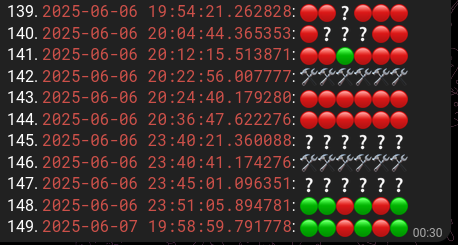
\includegraphics[width=0.5\textwidth]{images/memoria.png}
    \caption{Resultados de las partidas con las distintas heurísticas.}
    \label{fig:partidas_resultados}
\end{figure}


